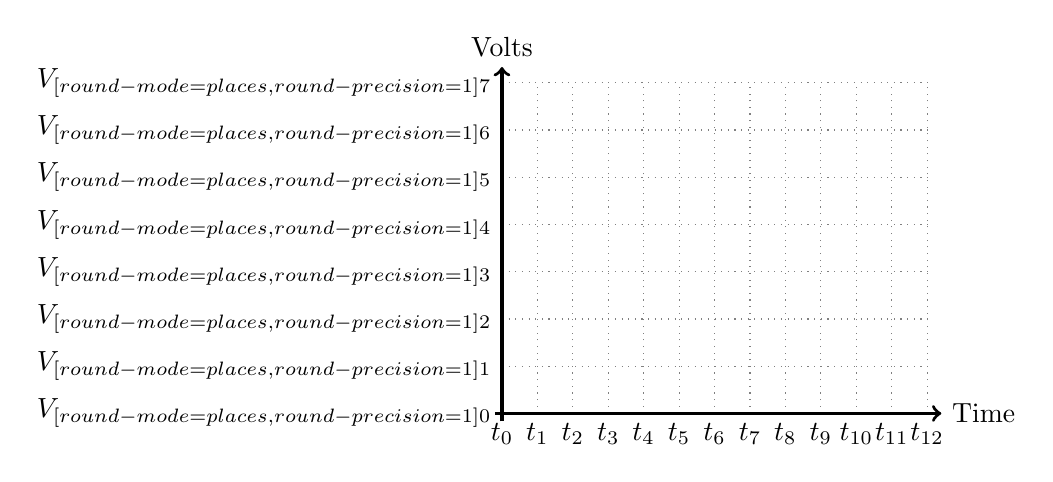
\begin{tikzpicture}[xscale=.9]
	% samples
	\draw[xstep=.5, ystep=.6, thin, color=gray, dotted] (0,0) grid (6, 4.2);

	% path
    \draw[thick] plot[id=sin,samples=1000,domain=0:6] function{-((x/2-1)**2)+4};

	% xtics
	\foreach \x in {0, ..., 12}
	{
		\draw ({\x/2}, 0) node[below] {$t_{\x}$};
	}

	% ytics
	\foreach \y in {0, 1, ..., 7.1}
	{
		\draw[thick] (0, .6*\y) node[left] {$V_{\num[round-mode=places, round-precision=1]{\y}}$};
	}

	% axes
    \draw[->, very thick] (-0.1,0) -- (6.2,0) node[right] {Time};
    \draw[->, very thick] (0,-.1) -- (0,4.4) node[above] {Volts};
\end{tikzpicture}
